\documentclass[11pt, twoside, pdftex]{article}

% This includes all the settings that we should use for the document
\newcommand{\PDFTitle}{Using Intel OpenCL\textsuperscript{\texttrademark} on DE-Series Boards}
\newcommand{\commonPath}{../../Common}
\newcommand{\datePublished}{Mar 2022}

\newcommand{\versnum}{21.1} %version number quartus/AMP
\newcommand{\quartusname}{Quartus\textsuperscript{\textregistered} Prime}	
\newcommand{\textBar}{For \quartusname{} \versnum{}}
\newcommand{\thisyear}{2022 } %for copyright
\newcommand{\company}{FPGAcademy.org}
\newcommand{\longteamname}{FPGAcademy.org}
\newcommand{\teamname}{FPGAcademy}
\newcommand{\website}{FPGAcademy.org}

\newcommand{\productAcronym}{AMP}
\newcommand{\productNameShort}{Monitor Program}

\newcommand{\productNameMedTM}{Monitor Program}
\newcommand{\productNameMed}{Monitor Program}

%\newcommand{\headerLogoFilePath}[1]{#1/FPGAcademy.png}



\setlength\topmargin{-0.25in}
\setlength\headheight{0in}
\setlength\headsep{0.35in}
\setlength\textheight{8.5in}
\setlength\textwidth{7in}
\setlength\oddsidemargin{-0.25in}
\setlength\evensidemargin{-0.25in}
\setlength\parindent{0.25in}
\setlength\parskip{0in} 

\pdfpagewidth 8.5in
\pdfpageheight 11in

% listings is a package that supports encapsulating source code in LaTeX conveniently

\usepackage{listings}
% add support for graphics
\usepackage{graphicx}
\usepackage[usenames, dvipsnames]{color}

\def\expandparam\lstinputlisting[#1]#2{\edef\tmp{\noexpand\lstinputlisting[#1]{#2}}\tmp}

\widowpenalty 10000
\clubpenalty 10000

%%%%%%%%%%%%%%%%%%%% Source Code Formatting %%%%%%%%%%%%%%%%%%%%
\definecolor{globalCommentColour}{rgb}{0.588,0.588,0.588}

%%%%%%%%%%%%%%%%%%%%%%%%%%%%%%%%%%%%%%%%%%%%%%%%%%%%
% Defining a NiosII ASM highlighter for lstlisting
\lstdefinelanguage[NiosII]{Assembler} {
 	morekeywords={add, addi, and, andhi, andi, beq, bge, bgeu, bgt, bgtu, ble,  bleu, blt, bltu, bne, br, break,% 
 	bret, call, callr, cmpeq, cmpeqi, cmpge, cmpgei, cmpgeu, cmpgeui, cmpgt, cmpgti, cmpgtu, cmpgtui, cmple,%
 	cmplei, cmpleu, cmpleui, cmplt, cmplti, cmpltu, cmpltui, cmpne, cmpnei, custom, div, divu, eret, flushd,%
 	flushda, flushi, flushp, initd, initda, initi, jmp, jmpi, ldb, ldbio, ldbu, ldbuio, ldh, ldhio, ldhu, ldhuio,%
 	ldw, ldwio, mov, movhi, movi, movia, movui, mul, muli, mulxss, mulxsu, mulxuu, nextpc, nop, nor, or, orhi, ori,%
 	rdctl, rdprs, ret, rol, roli, ror, sll, slli, sra, srai, srl, srli, stb, stbio, sth, sthio, stw, stwio,%
 	sub, subi, sync, trap, wrctl, wrtcl, wrprs, xor, xori, xorhi, xori},% 	
 	morekeywords=[2]{.abort, .ABORT, .align, .app-file, .ascii, .asciz, .balign, .byte, .comm, .data, .def,%
 	.desc, .dim, .double, .eject, .else, .end, .endef, .endif, .equ, .equiv, .err, .extern, .file, .fill, .float,%
 	.global, .globl, .hword, .ident, .if, .include, .int, .irp, .irpc, .lcomm, .lflags, .line, .linkonce, .ln,%
 	.list, .long, .macro, .mri, .nolist, .octa, .org, .p2align, .psize, .quad, .rept, .sbttl, .scl, .section,%
 	.set, .short, .single, .size, .sleb128, .skip, .space, .stadb, .stabn, .stabs, .string, .symver, .tag,%
 	.text, .title, .type, .val, .uleb128, .word},% 	
 	morekeywords=[3]{et, bt, gp, sp, fp, ea, sstatus, ra, pc, status, estatus, bstatus, ienable, ipending, cpuid,%
 	exception, pteaddr, tlbacc, tlbmisc, eccinj, badaddr, config, mpubase, mpuacc},% 	
 	sensitive=t,%
 	alsoletter=.,%
	morestring=[b]",%
 	morecomment=[s]{/*}{*/},%
 	morecomment=[l]\#,%
   }[keywords,comments,strings]
   
   %% NOTE: morekeywords=[2] are GNU directives.
   
   \definecolor{niosInstructionColour}{rgb}{0.000,0.608,0.000}
   \definecolor{niosDirectiveColour}{rgb}{0.000,0.000,0.902}
   \definecolor{niosSpecialRegColour}{rgb}{0.000,0.000,0.000}
   \definecolor{niosStringColour}{rgb}{0.808,0.482,0.000}
   
   %% NOTE: To make bold use: =\bfseries\color{<colour>}
   \lstdefinestyle{defaultNiosStyle} {
   language=[NiosII]{Assembler},
   stringstyle=\color{niosStringColour},
   keywordstyle=\color{niosInstructionColour},
   keywordstyle=[2]\color{niosDirectiveColour},
   keywordstyle=[3]\itshape\color{niosSpecialRegColour}
   }
%%%%%%%%%%%%%%%%%%%%%%%%%%%%%%%%%%%%%%%%%%%%%%%%%%%%

%%%%%%%%%%%%%%%%%%%%%%%%%%%%%%%%%%%%%%%%%%%%%%%%%%%%
% Defining a ArmA9 ASM highlighter for lstlisting
\lstdefinelanguage[ArmA9]{Assembler} {
 	morekeywords={ADC, ADD, ADDS, AND, ANDS, B, BAL, BEQ, BGE, BGT, BL, BLT, BIC, BKPT, BLX, BNE, BX, CDP, CLZ, CMN, CMP, EOR,%
 	EORS, LDC, LDM, LDR, LDRB, LDRBT, LDRH, LDRSB, LDRSH, LDRT, LSL, MCR, MLA, MOV, MOVW, MOVT, MRC, MRS, MSR, MUL, MVN, ORR, PLD,%
 	ROR, RSB, RSC, SBC, SMLAL, SMULL, STC, STM, STR, STRB, STRBT, STRH, STRT, SUB, SUBS, SWI, SWP, SWPB, TEQ, UMLAL,
 	PUSH, POP, MOVS, RORS, LSR},%
 	morekeywords=[2]{.abort, .ABORT, .align, .app-file, .ascii, .asciz, .balign, .byte, .comm, .data, .def,%
 	.desc, .dim, .double, .eject, .else, .end, .endef, .endif, .equ, .equiv, .err, .extern, .file, .fill, .float,%
 	.global, .globl, .hword, .ident, .if, .include, .int, .irp, .irpc, .lcomm, .lflags, .line, .linkonce, .ln,%
 	.list, .long, .macro, .mri, .nolist, .octa, .org, .p2align, .psize, .quad, .rept, .sbttl, .scl, .section,%
 	.set, .short, .single, .size, .sleb128, .skip, .space, .stadb, .stabn, .stabs, .string, .symver, .tag,%
 	.text, .title, .type, .val, .vectors, .uleb128, .word},%
 	morekeywords=[3]{SP, PC, MIDR, CTR, TCMTR, TLBTR, MPIDR, ID_PFR0, ID_PFR1, ID_DFR0, ID_MMFR0, ID_MMFR1, ID_MMFR2,%
 	ID_MMFR3, ID_ISAR0, ID_ISAR1, ID_ISAR2, ID_ISAR3, ID_ISAR4, CCSIDR, CLIDR, AIDR, CSSELR, TTBR0, TTRB1, TTBR2, DACR,%
 	DFSR, IFSR, ADFSR, AIFSR, DFAAR, IFAR, ICIALLUIS, BPIALLIS, PAR, ICIALLU, ICIMVAU, BPIALL, DCIMVAC, DCISW, V2PCWPR,%
 	DCCVAC, DCCSW, DDIMVAC, DCISW, TLBALLIS, TLBIMVAIS, TLBIASIDIS, TLBIMVAAIS, TLBIALL, TLBIMVA, TLBIASID, TLBIMVAA,%
 	PMCR, PMCNTENSET, PMCNTENCLR, PMOVSR, PMSWINC, PMSELR, PMXEVTYPER, PMXEVCNTR, PMUSERENR, PMINTENSET, PMINTENCLR,%
 	PRRR, NRRR, PLEIDR, PLEASR, PLEFSR, PLEUAR, PLEPCR, VBAR, MVBAR, ISR, FCSEIDR, CONTEXTIDR, TPIDRURW, TPIDRURO, TPIDRPRW},%
 	sensitive=f,%
 	alsoletter=.,%
	morestring=[b]",%
 	morecomment=[s]{/*}{*/},%
 	morecomment=[l]{//},%
   }[keywords,comments,strings]
   
   %% NOTE: morekeywords=[2] are GNU directives.
   
   \definecolor{armInstructionColour}{rgb}{0.000,0.608,0.000}
   \definecolor{armDirectiveColour}{rgb}{0.000,0.000,0.902}
   \definecolor{armSpecialRegColour}{rgb}{0.000,0.000,0.000}
   \definecolor{armStringColour}{rgb}{0.808,0.482,0.000}
   
   \lstdefinestyle{defaultArmStyle} {
   language=[ArmA9]{Assembler},
   stringstyle=\color{armStringColour},
   keywordstyle=\color{armInstructionColour},
   keywordstyle=[2]\color{armDirectiveColour},
   keywordstyle=[3]\itshape\color{armSpecialRegColour}
   }
%%%%%%%%%%%%%%%%%%%%%%%%%%%%%%%%%%%%%%%%%%%%%%%%%%%%

%%%%%%%%%%%%%%%%%%%%%%%%%%%%%%%%%%%%%%%%%%%%%%%%%%%%
% Defining style for the verilog.

\definecolor{verilogCommentColour}{rgb}{0.000,0.502,0.000}

\lstdefinestyle{defaultVerilogStyle} {
language={Verilog},
keywordstyle=\color{blue},
commentstyle=\color{verilogCommentColour}
}
%%%%%%%%%%%%%%%%%%%%%%%%%%%%%%%%%%%%%%%%%%%%%%%%%%%%

%%%%%%%%%%%%%%%%%%%%%%%%%%%%%%%%%%%%%%%%%%%%%%%%%%%%
% Defining style for the vhdl.
\lstdefinestyle{defaultVHDLStyle} {
language={VHDL},
keywordstyle=\color{blue},
commentstyle=\color{verilogCommentColour}
}
%%%%%%%%%%%%%%%%%%%%%%%%%%%%%%%%%%%%%%%%%%%%%%%%%%%%

%%%%%%%%%%%%%%%%%%%%%%%%%%%%%%%%%%%%%%%%%%%%%%%%%%%%
% Java
\definecolor{javaStringColour}{rgb}{0.808,0.482,0}
%%%%%%%%%%%%%%%%%%%%%%%%%%%%%%%%%%%%%%%%%%%%%%%%%%%%

%%%%%%%%%%%%%%%%%%%%%%%%%%%%%%%%%%%%%%%%%%%%%%%%%%%%
% Defining language styles
% C
\definecolor{CStringColour}{rgb}{0.808,0.482,0}
%%%%%%%%%%%%%%%%%%%%%%%%%%%%%%%%%%%%%%%%%%%%%%%%%%%%

%%%%%%%%%%%%%%%%%%%%%%%%%%%%%%%%%%%%%%%%%%%%%%%%%%%%
% Defining extended LaTeX language.
\lstdefinelanguage[LocalLaTeX]{TeX}[LaTeX]{TeX}%
 	{moretexcs={bf, it, sf, lstset},%
   	}%

\lstdefinestyle{defaultLocalLatexStyle} {
language=[LocalLatex]{TeX},
keywordstyle=\color{blue}\bfseries,
keywordstyle=[2]\color{blue},
keywordstyle=[3]\color{blue}\bfseries
}
%%%%%%%%%%%%%%%%%%%%%%%%%%%%%%%%%%%%%%%%%%%%%%%%%%%%

\lstset{
%language = C,
%language = Verilog,
%basicstyle=\color{black}\rmfamily\ttfamily,
basicstyle=\small\color{black}\ttfamily,
commentstyle=\small\color{globalCommentColour}\itshape\ttfamily,
keywordstyle=\small\color{blue}\bfseries\ttfamily,
showstringspaces=false,
frame=none, %lines % boxed listings
breaklines=true,
breakatwhitespace=true,
tabsize=4
}
%%%%%%%%%%%%%%%%%%%%%%%%%%%%%%%%%%%%%%%%%%%%%%%%%%%%%%%%%%%%%%%%


%\usepackage[centering]{geometry}.
%%%%%%%%%%%%%%%%%%%%%%%%%%%%%%%%%%%%%%%%%%%%%%%%%%%
% Document Settings
\usepackage[labelsep=period]{caption}
% we can choose a better font later
%\usepackage{palatino}
\usepackage{fourier}
%\fontencoding{T1}
% include common used symbols
\usepackage{textcomp}
% add support for graphics
\usepackage{graphicx}
\usepackage[usenames, dvipsnames]{color}
% enable to draw thick or thin table hlines
\setlength{\doublerulesep}{\arrayrulewidth}
\usepackage{longtable}
\setlongtables
%\usepackage{array}
% It may be better to use PDFLaTeX as it can generate bookmarks for the
% document

% Add some useful packages
\usepackage{ae,aecompl}
\usepackage{epsfig,float,times}

% reset the font for section
\usepackage{sectsty}
%\allsectionsfont{\fontfamily{ptm}\selectfont}
\allsectionsfont{\usefont{OT1}{phv}{bc}{n}\selectfont}

% use compact space for sections
\usepackage[compact]{titlesec}
\titlespacing{\section}{0pt}{0.2in}{*0}
\titlespacing{\subsection}{0pt}{0.1in}{*0}
\titlespacing{\subsubsection}{0pt}{0.05in}{*0}

% fancyhdr header and footer customization
\usepackage{layout}
\usepackage{fancyhdr}
\pagestyle{fancy}
\fancyhead{}
\fancyhead[R]{\textit{\tiny{\textBar}}}
\fancyfoot{}
\fancyfoot[LO,
RE]{\textrm{\href{https://www.fpgacademy.org}{\small \longteamname}} \\ {\small \datePublished }}
\fancyfoot[RO, LE]{\small \thepage}
% two-side settings
%\fancyhead{} % clear all header fields
%\fancyfoot{} % clear all footer fields
%\fancyfoot[LE,RO]{\thepage}
\renewcommand{\headrulewidth}{2pt}
\renewcommand{\headrule}{{\color{blue} \hrule width\headwidth height\headrulewidth \vskip-\headrulewidth}}
\renewcommand{\footrulewidth}{0pt}

% Format the footer on page 1
\fancypagestyle{plain}{
\fancyhead{}
\fancyfoot{}
\fancyfoot[LO,
RE]{\textrm{\href{https://www.fpgacademy.org}{\small \longteamname}} \\ {\small \datePublished }}
\fancyfoot[RO, LE]{\small \thepage}
\renewcommand{\headrulewidth}{0pt}
}
% adjust some setting to try to make the figure stay in the same page with text
% Reference: 	http://www.cs.uu.nl/~piet/floats/node1.html
%   			http://mintaka.sdsu.edu/GF/bibliog/latex/floats.html
%   General parameters, for ALL pages:
\renewcommand{\topfraction}{0.9}	% max fraction of floats at top
\renewcommand{\bottomfraction}{0.8}	% max fraction of floats at bottom
%   Parameters for TEXT pages (not float pages):
\setcounter{topnumber}{3}
\setcounter{bottomnumber}{3}
\setcounter{totalnumber}{5}     % 2 may work better
\setcounter{dbltopnumber}{2}    % for 2-column pages
\renewcommand{\dbltopfraction}{0.9}	% fit big float above 2-col. text
\renewcommand{\textfraction}{0.07}	% allow minimal text w. figs
%   Parameters for FLOAT pages (not text pages):
\renewcommand{\floatpagefraction}{0.7}	% require fuller float pages
% N.B.: floatpagefraction MUST be less than topfraction !!
\renewcommand{\dblfloatpagefraction}{0.7}	% require fuller float pages
%%%%%%%%%%%%%%%%%%%%%%%%%%%%%%%%%%%%%%%%%%%%%%%%%%%
% remember to use [htp] or [htpb] for placement
%%%%%%%%%%%%%%%%%%%%%%%%%%%%%%%%%%%%%%%%%%%%%%%%%%%

% set no indent for paragraph
\setlength{\parindent}{0em}
\addtolength{\parskip}{11pt}
\newcommand{\compact}{[topsep=0pt]}
% use this package to reduce space
\usepackage{enumitem}
\usepackage{multirow}
\usepackage{rotating}
\usepackage{pifont}
\usepackage{dingbat}
\newcommand{\itemsecond}{$\circ$}
%
%%%%%%%%%%%%%%%%%%
\date{}
\author{}
%%%%%%%%%%%%%%%%%%
\newcommand{\de}{DE-series}
\newcommand{\up}{FPGAcademy}
\newcommand{\fabric}{Avalon Switch Fabric}
\newcommand{\TODO}[1]{\textcolor{red}{\textbf{TODO}: #1}}
\def\registered{{\ooalign{\hfil\raise .00ex\hbox{\scriptsize R}\hfil\crcr\mathhexbox20D}}}

% enable url and reference(bookmarks) in pdf
\usepackage{url}
\usepackage[pdftex, colorlinks]{hyperref}
\hypersetup{%
pdftitle={\PDFTitle},
linkcolor=blue,
hyperindex=true,
pdfauthor={\longteamname},
pdfkeywords={FPGAcademy, Academic Program, Example System},
bookmarksnumbered,
bookmarksopen=false,
filecolor=blue,
pdfstartview={FitH},
urlcolor=blue,
plainpages=false,
pdfpagelabels=true,
linkbordercolor={1 1 1} %no color for link border
}%
%%%%%%%%%%%%%%%%%%%%%%%%%%%%%%%%%%%%%%%%%%%%%%%%%%%
\setlength{\fboxsep}{0.7pt}
\setlength{\fboxrule}{0.5pt}

\newcommand{\red}[1]{{\color{red}\sf{#1}}}
\newcommand{\blue}[1]{{\color{blue}\sf{#1}}}



\usepackage{placeins}
\usepackage{listings}
\usepackage{hyperref}

%%%%%%%%%%%%%%%%%%%%%%%%%
% Add title
\newcommand{\doctitle}{Using Intel FPGA SDK for OpenCL\textsuperscript{\texttrademark} on DE-Series Boards}
\newcommand{\dochead}{Using Intel FPGA SDK for OpenCL\textsuperscript{\texttrademark} on DE-Series Boards}
% Usually no need to change these two lines
\title{\fontfamily{phv}\selectfont{\doctitle} }
\chead{ \small{\textsc{\bfseries \dochead} } }
% Customizations
%%%%%%%%%%%%%%%%%%%%%%%%%
% Allows multiple figures per page

\renewcommand\floatpagefraction{.9}
\renewcommand\topfraction{.9}
\renewcommand\bottomfraction{.9}
\renewcommand\textfraction{.1}   
\setcounter{totalnumber}{50}
\setcounter{topnumber}{50}
\setcounter{bottomnumber}{50}
\raggedbottom

%%%%%%%%%%%%%%%%%%
%%% DOCUMENT START
%\begin{document}
\begin{document}
\begin{table}
    \centering
    \begin{tabular}{p{5cm}p{4cm}}
        \hspace{-3cm}
        &
        \raisebox{1\height}{\parbox[h]{0.5\textwidth}{\Large\fontfamily{phv}\selectfont{\textsf{\doctitle}}}}
    \end{tabular}
    \label{tab:logo}
\end{table}

\colorbox[rgb]{0,0.384,0.816}{\parbox[h]{\textwidth}{\color{white}\textsf{\textit{\textBar}}}}

\thispagestyle{plain}

\section{Introduction}

This tutorial provides a brief introduction to OpenCL\textsuperscript{\texttrademark} and the Intel\textsuperscript{\textregistered} FPGA SDK for OpenCL, and describes how to compile and execute OpenCL applications that target SoC-based DE-series boards such as the DE10-Standard, DE10-Nano, and DE1-SoC.\\
\\
{\bf Contents:}
\begin{itemize}
\item Overview of OpenCL
\item Overview of Intel FPGA SDK for OpenCL
\item Compiling a Sample OpenCL Application
\item Executing an OpenCL Application on DE-Series Boards
\end{itemize}

{\bf Requirements:}

\begin{itemize}
%\item Intel Quartus software
\item Familiarity with using Linux* on DE-series boards, which can be achieved by reading the tutorial \textit{Using Linux on DE-Series Boards}
%\item The \textit{arm-linux-gnueabihf-} compiler toolchain (available with Intel SoC EDS or separately online)
\end{itemize}

\clearpage
\newpage

\section{What is OpenCL\textsuperscript{\texttrademark}?}

OpenCL is a C-based programming language designed for writing applications that run on heterogeneous compute platforms. These platforms generally consist of different compute devices such as CPUs, GPUs, and FPGAs. Traditionally, each of these devices has had its own methods for programming. As an example, a developer might have had to write C code for the CPU, OpenGL code for the GPU, and Verilog code for the FPGA. In contrast, a developer can use OpenCL to create a single application that executes across all of the devices. This makes it easier to extract performance out of heterogeneous systems, using each device's unique strengths to speed up corresponding portions of the application.

OpenCL has a number of key features that make it suited for programming heterogeneous systems. First, OpenCL provides an abstraction layer for programming the devices in the system. This means that device-specific details are hidden to the developer which makes writing code easier, especially if the developer does not have a deep understanding of the devices. The abstraction also means their application code is not specific to certain devices, architectures, or vendors, leaving them free to migrate their application to newer platforms.  Second, OpenCL allows developers to specify parallelism in in fine detail. As a typical heterogeneous system contains parallel accelerators such as GPUs and FPGAs, it is important to be able to write parallelized applications that make effective use of these devices.

An OpenCL application is split into two parts, the \textbf{host program} and the \textbf{kernel(s)}. The host program is executed on the CPU of the system, and can perform any functions or computations as if it were a regular C program. In addition, an OpenCL host program is able to launch one or more kernels in order to speed up computation. A \textbf{kernel} is a special function written in OpenCL C that performs some user-defined computation. The kernel is executed on an accelerator device such as an FPGA. Often, the kernel is designed to perform some computation that can be executed in parallel - in order to effectively leverage the parallel nature of an accelerator like the FPGA. As an example, consider matrix addition of two m x n matrices. Here, we could design the kernel to do a single addition (between two corresponding matrix cells), allowing for any number of kernels between 1 to m x n to execute in parallel. While a CPU would take m x n cycles to do this matrix addition, an FPGA containing many of these kernels could compute the operation in parallel, thereby speeding up the application.

This tutorial is not intended to be a comprehensive guide to the OpenCL language nor the Intel FPGA SDK for OpenCL. Instead, this tutorial provides the minimal information necessary to start using OpenCL on the DE-Series boards. For more information about writing OpenCL and using the Intel FPGA SDK for OpenCL, please refer to the documents listed below:

\begin{itemize}
\item \href{https://www.altera.com/documentation/mwh1391807309901.html}{Intel FPGA SDK for OpenCL Getting Started Guide}
\item \href{https://www.altera.com/documentation/mwh1391807516407.html}{Intel FPGA SDK for OpenCL Programming Guide}
\item \href{https://www.altera.com/documentation/mwh1391807965224.html}{Intel FPGA SDK for OpenCL Best Practices Guide}
\end{itemize}

\textbf{Note:} This tutorial will use the DE10-Standard board as a reference, but the procedure is almost identical for other DE-series boards.

\pagebreak

\section{Introduction to the Intel\textsuperscript{\textregistered} FPGA SDK for OpenCL\textsuperscript{\texttrademark}}

The Intel FPGA SDK for OpenCL can be used to compile OpenCL applications that target heterogeneous systems containing Intel FPGA(s). Such a system contains a CPU, such as an x86 or ARM* processor, and one or more Intel FPGAs. For x86-based systems, the FPGA typically resides on an FPGA accelerator board, which is connected to the system through the PCIe interface. For SoC-FPGA systems, the FPGA is generally connected to the processor through specialized bridges, as is the case with Intel SoC-FPGA devices found on DE-series Boards. The host program of the OpenCL application executes on the CPU, and the kernels are placed into the FPGA and launched on-demand by the host program. 

The Intel FPGA SDK for OpenCL provides the tools required to allow the implementation of OpenCL applications that target Intel FPGAs. Three main components comprise the SDK: 

\begin{itemize}
\item The \textit{Intel Offline Compiler} (AOC) which translates the OpenCL kernel code into hardware that can be programmed onto the FPGA.
\item The \textit{host runtime} which is a collection of libraries and drivers that allow the host program to communicate with the kernel(s) in the FPGA.
\item The \textit{AOCL} utility which provides a set of commands to perform tasks such as downloading the kernel into the FPGA and running diagnostics to check that OpenCL drivers have been initialized.
\end{itemize}

The developer uses the Intel FPGA SDK for OpenCL in conjunction with a standard C++ compiler to compile the OpenCL application. Figure~\ref{fig:altera_sdk_flow} shows the compilation and execution flow at a high level. The flow is described in more detail below:

\begin{enumerate}
\item The developer writes their OpenCL application code, which consists of a host program written in C/C++, and kernel(s) written in OpenCL C.
\item The developer compiles the OpenCL application:
\begin{enumerate}
\item The host program is compiled via GCC or Visual Studio, linking in the Intel OpenCL host runtime libraries. This creates the host program binary to be executed by the CPU.
\item The kernel(s) are compiled via the AOC. This creates the Intel OpenCL Executable (.aocx) file, which can be downloaded onto the FPGA. %The host program is then able to communicate with the FPGA and launch these kernels.
\end{enumerate}
\item The developer uses the AOCL utility to load the .aocx programming file onto the FPGA. The FPGA now contains the kernel(s) that will be launched by the host program.
\item The OpenCL application is executed by running the host program. Throughout its execution, the host program launches the FPGA kernels as needed.  %The host program is able to launch the FPGA kernels, by communicating through the 
\end{enumerate}

\begin{figure} [H]
\begin{center}
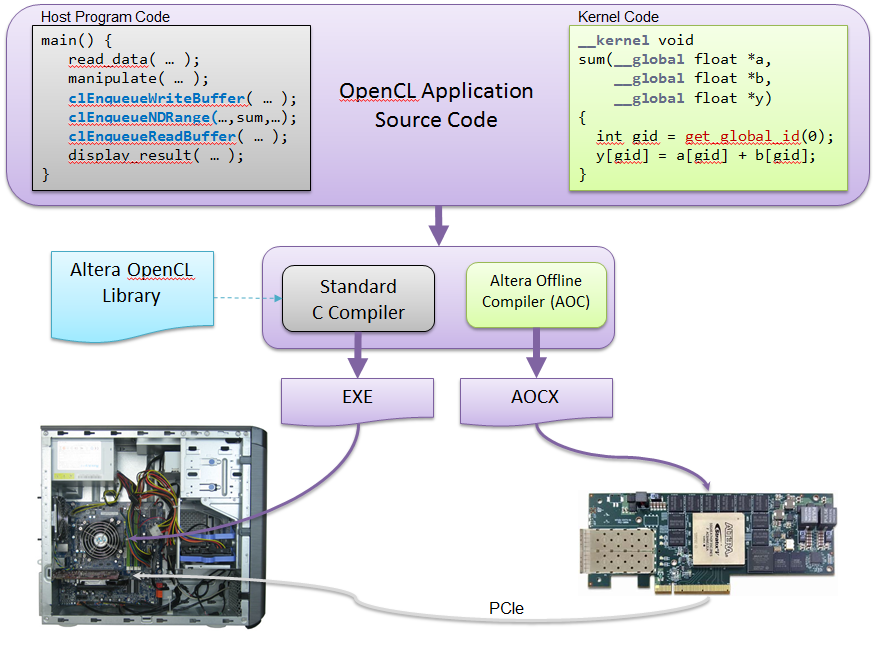
\includegraphics[scale = 0.7]{figures/flow.png}
\end{center}
\caption{The Intel FPGA SDK for OpenCL Flow}
\label{fig:altera_sdk_flow}
\end{figure}

\subsection{Installing the Intel\textsuperscript{\textregistered} FPGA SDK for OpenCL\textsuperscript{\texttrademark}}
\label{sec:install_sdk}

To install the Intel FPGA SDK for OpenCL on your host computer, follow the instructions below. The Intel FPGA SDK for OpenCL
also installs the required Intel Quartus\textsuperscript{\textregistered} Prime software. You do not have to install Quartus Prime software separately. 

\begin{enumerate}
%\item Go to DE-series board section on Terasic's website (\url{https://www.terasic.com.tw/en/}).
%\item Find the DE-series board you are using and click on it.
%\item Go to the \textit{Resources} tab and scroll down to find the \textbf{Board Support Package for Intel FPGA SDK OpenCL} for your board.
%\item \textbf{You do not need to download the BSP yet}. Take note of the OpenCL SDK version used to build this board package (BSP). For the DE10-Standard, version 16.1 was used.
%	\begin{figure} [H]
%	\begin{center}
%	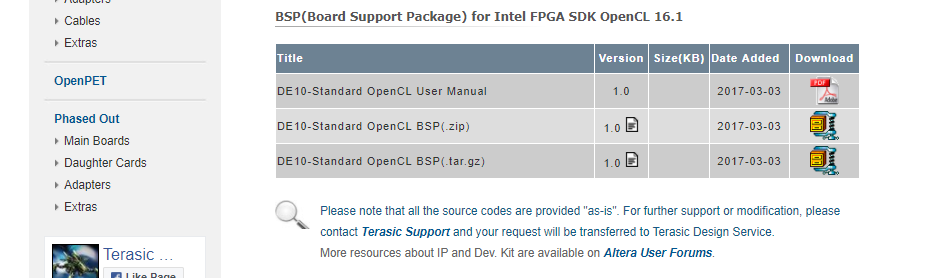
\includegraphics[scale = 0.7]{figures/fig_terasic_bsp_download.png}
%	\end{center}
%	\caption{Terasic's Board Support Package version and download}
%	\label{fig:terasic_bsp_download_1}
%	\end{figure}
\item Go to \url{http://dl.altera.com/opencl/}.
\item Select either the PRO or STANDARD edition of the SDK depending on the device family that you wish to target. To determine which version is appropriate for your device you can consult the table at \url{https://dl.altera.com/devices/}. 

%		Note: If you plan to target Arria or Stratix 10 devices you should select the PRO edition, otherwise select the STANDARD edition.
%\item \textbf{For versions 17.0 and later}: Select either the PRO or STANDARD depending on your needs.
%\item \textbf{For versions 16.1 and earlier}: The version is selected after download.
	\begin{figure} [H]
	\begin{center}
	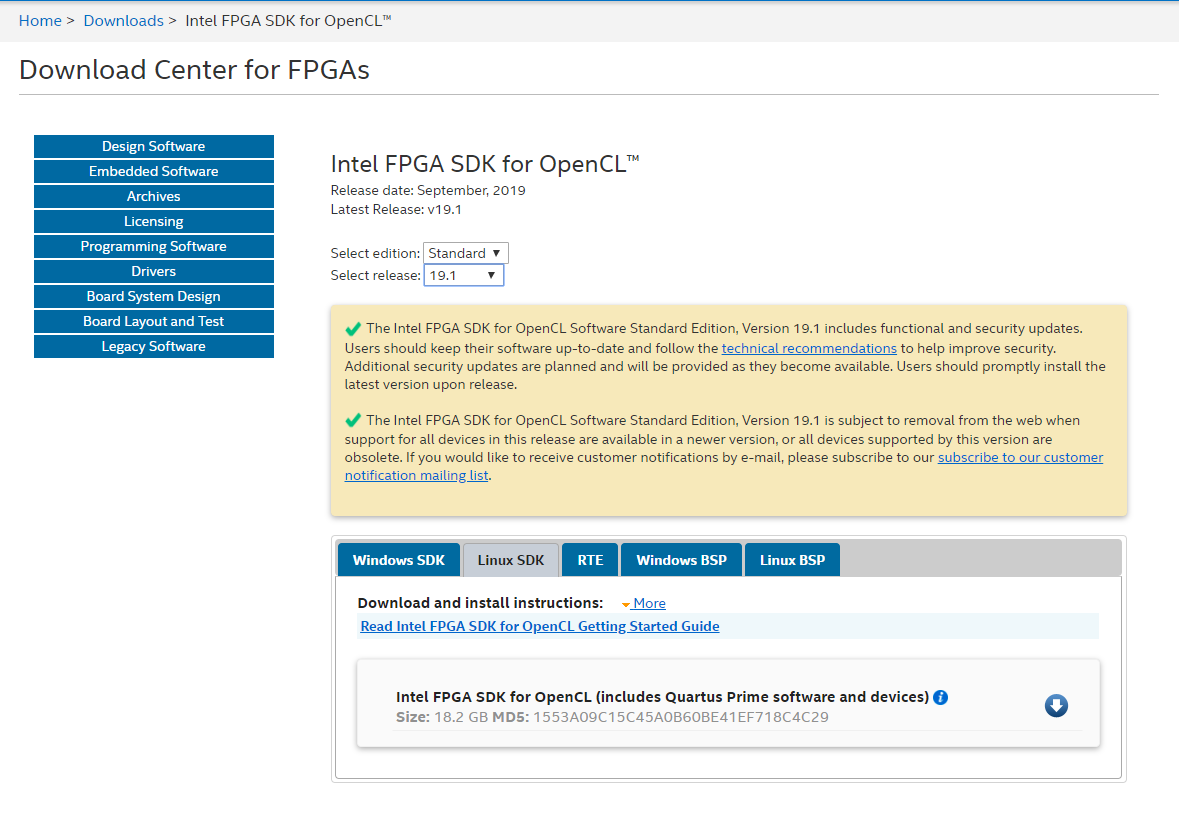
\includegraphics[scale = 0.5]{figures/fig_download_ocl_sdk.png}
	\end{center}
	\caption{Intel FPGA SDK for OpenCL Download}
	\label{fig:intel_ocl_sdk_download}
	\end{figure}
\item Download the \textit{Windows* SDK} or the \textit{Linux SDK} depending on your operating system. This will download a large TAR file and may take a long time to complete.
%	\begin{figure} [H]
%	\begin{center}
%	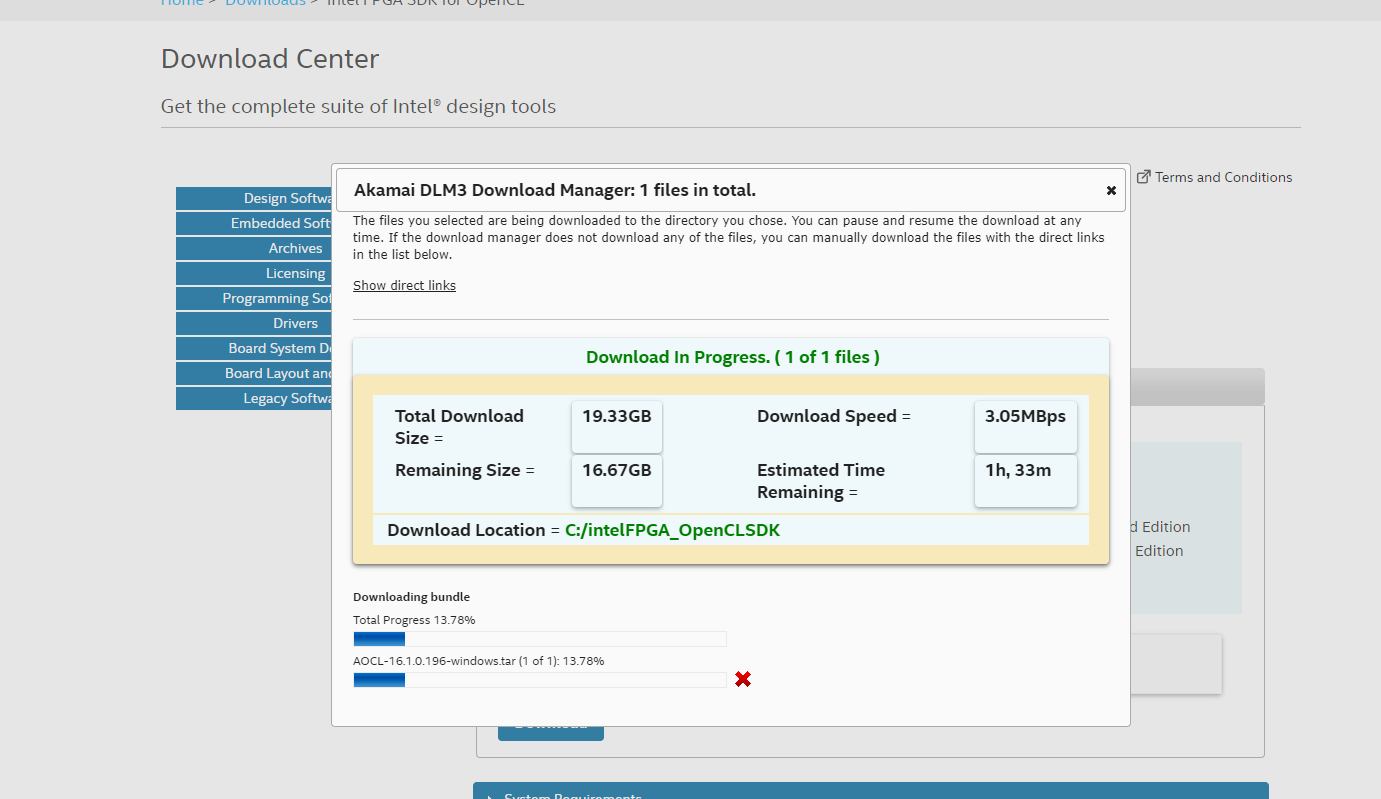
\includegraphics[scale = 0.3]{figures/fig_akamai_download.png}
%	\end{center}
%	\caption{Akamai Download Manager - Intel FPGA SDK for OpenCL}
%	\label{fig:akamai_download_manager}
%	\end{figure}
\item Extract the contents of the TAR file.
\item Run the installer:
\subitem On Windows, double click the \textit{setup.bat} file. 
\subitem On Linux, open a terminal, \texttt{cd} to the extracted files, then run the command \texttt{sudo ./setup.sh}.

The installer GUI will appear, as shown in Figure~\ref{fig:quartus_install_1}.
%\item If you require the PRO edition and downloaded \textbf{version 16.1 or earlier} run the \textit{setup\_pro.bat} file.
\item Follow the instructions in the installer GUI to install the SDK. At the step shown in Figure~\ref{fig:quartus_install_2}, take note of the directory where the SDK is being installed. The installer comes with support for a variety of FPGA device families. To save disk space, you can choose to install only the device(s) that you you need as shown in Figure~\ref{fig:quartus_install_3}. 
	\begin{figure} [H]
	\begin{center}
	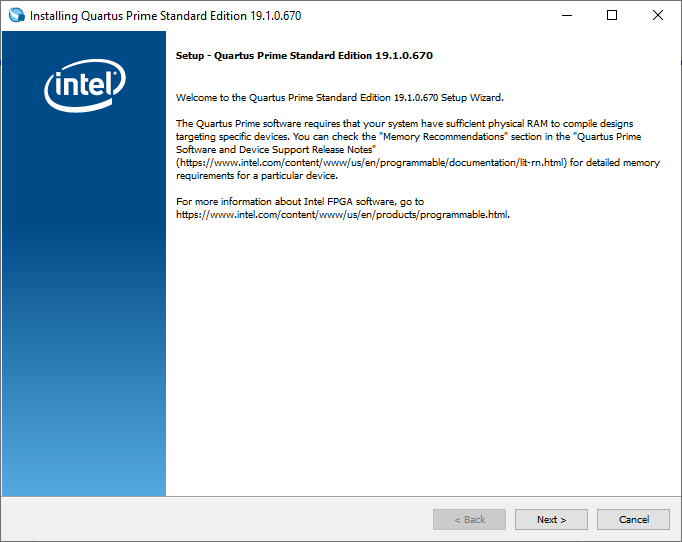
\includegraphics[scale = 0.7]{figures/fig_install_1.png}
	\end{center}
	\caption{Quartus Installation}
	\label{fig:quartus_install_1}
	\end{figure}
	
	\begin{figure} [H]
	\begin{center}
	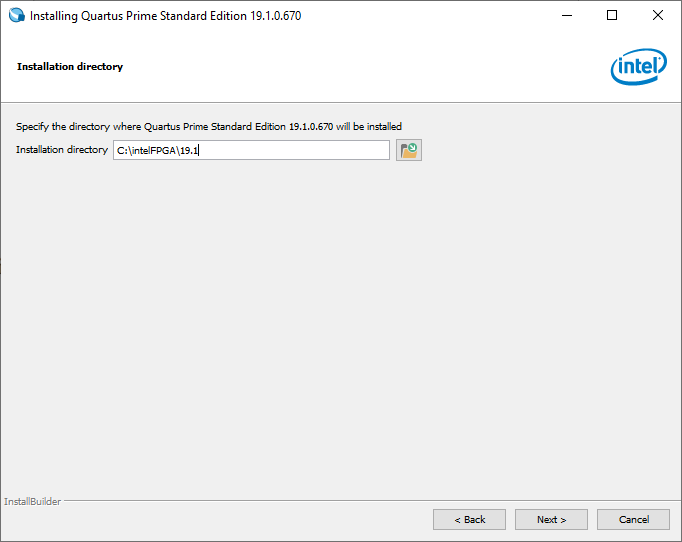
\includegraphics[scale = 0.7]{figures/fig_install_2.png}
	\end{center}
	\caption{Quartus Installation - Selecting the Quartus Root Directory}
	\label{fig:quartus_install_2}
	\end{figure}
	
	\begin{figure} [H]
	\begin{center}
	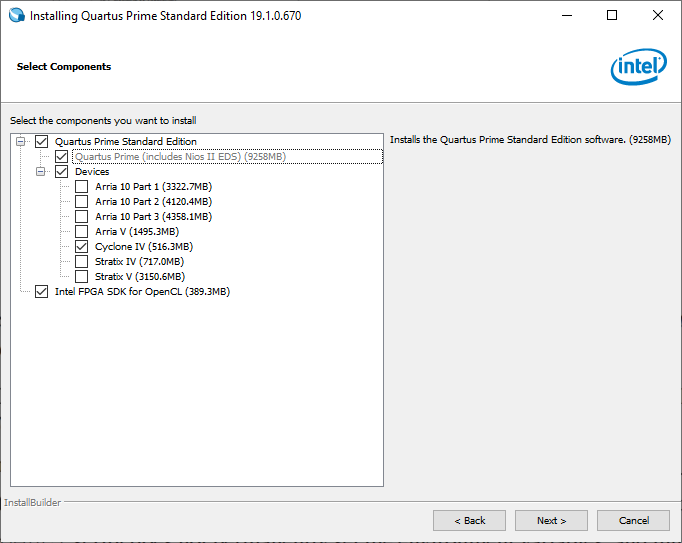
\includegraphics[scale = 0.7]{figures/fig_install_3.png}
	\end{center}
	\caption{Quartus Installation - Selecting FPGA Devices}
	\label{fig:quartus_install_3}
	\end{figure}
\item Once the installation completes, the Intel FPGA SDK for OpenCL will reside in \textit{<quartus root>/hld/} where \textit{<quartus root>} is the directory you chose in Figure~\ref{fig:quartus_install_2}.
%\item The installer automatically defines the path \path{QUARTUSROOT\hld\} to the environment variable \path{ALTERAOCLSDKROOT}.
%\item Next you must add the following paths to your \textit{PATH} environment variable (Note the \% symbols):
%	\begin{itemize}
%		\item \path{%ALTERAOCLSDKROOT%\bin}
%		\item \path{%ALTERAOCLSDKROOT%\windows64\bin}
%		\item \path{%ALTERAOCLSDKROOT%\host\windows64\bin}
%	\end{itemize}
%	For instructions on editing and adding environment variables see \nameref{sec:appendix_a}.
\item Before you can call SDK commands, you must set your operating system's environment variables to point to the new installation. You can do this as follows:
\subitem On Windows, open a CMD prompt and run the command \texttt{<quartusroot>\textbackslash hld\textbackslash init\_opencl.bat}.
\subitem On Linux, open a terminal and run the command \texttt{source <quartusroot>/hld/init\_opencl.sh}.

Note that the \texttt{init\_opencl} script does not permanently set the environment variables, and must be run each time you open a new CMD prompt or terminal. %If you would like to permanently set the environment variables, you must set the variables below:

%\subitem set \texttt{INTELFPGAOCLSDKROOT} to <quartusroot>/hld/
%\subitem append 

\item Verify the installation and environment variables by checking the output of the command \texttt{aocl version}.
The command should produce a version number output similar to Figure~\ref{fig:verify_intel_ocl_sdk}. 

	\begin{figure} [H]
	\begin{center}
	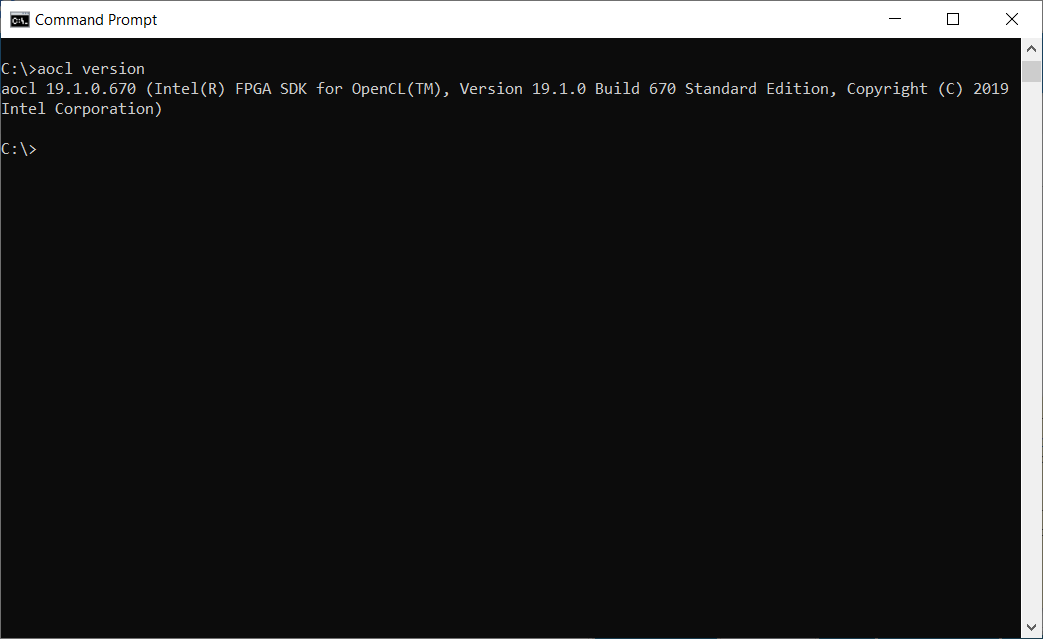
\includegraphics[scale = 0.5]{figures/fig_aocl_version.png}
	\end{center}
	\caption{Verifying Intel OpenCL SDK install}
	\label{fig:verify_intel_ocl_sdk}
	\end{figure}
\end{enumerate}

For more instructions on installing the Intel FPGA SDK for OpenCL, please refer to the document \href{https://www.altera.com/documentation/mwh1391807309901.html}{Intel FPGA SDK for OpenCL Getting Started Guide}.

\subsection{Installing the DE-Series Board Support Package}
\label{sec:install_bsp}

To compile OpenCL kernels for your DE-series board, you must install and use the corresponding board support package (BSP). To install the BSP, follow these instructions:

\begin{enumerate}
\item Go to DE-series board section on Terasic's website (\url{https://www.terasic.com.tw/en/}).
\item Go to the webpage for your board.
\item Go to the \textit{Resources} tab and scroll down to find the \textbf{BSP(Board Support Package) for Intel FPGA SDK OpenCL} for your board, as shown in Figure~\ref{fig:terasic_bsp_download_2}.
	\begin{figure} [H]
	\begin{center}
	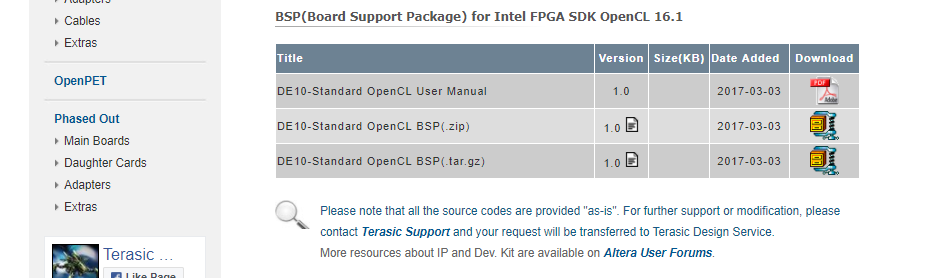
\includegraphics[scale = 0.7]{figures/fig_terasic_bsp_download.png}
	\end{center}
	\caption{Terasic's Board Support Package version and download}
	\label{fig:terasic_bsp_download_2}
	\end{figure}
%\item Copy the sub-directory (in the extracted directory) to \textit{QUARTUSROOT/hld/board/}. You should have a folder as shown in Figure~\ref{fig:move_bsp_download} for the DE10-Standard BSP. 
	%Note: \path{ALTERAOCLSDKROOT} is equivilant to \path{QUARTUSROOT\hld}).
\item Download the OpenCL BSP and extract its contents to \textit{<quartusroot>/hld/board/}. Figure~\ref{fig:move_bsp_download} shows the result of extracting the BSP contents for the DE10-Standard board to \textit{<quartusroot>/hld/board/}.
%	\begin{figure} [H]
%	\begin{center}
%	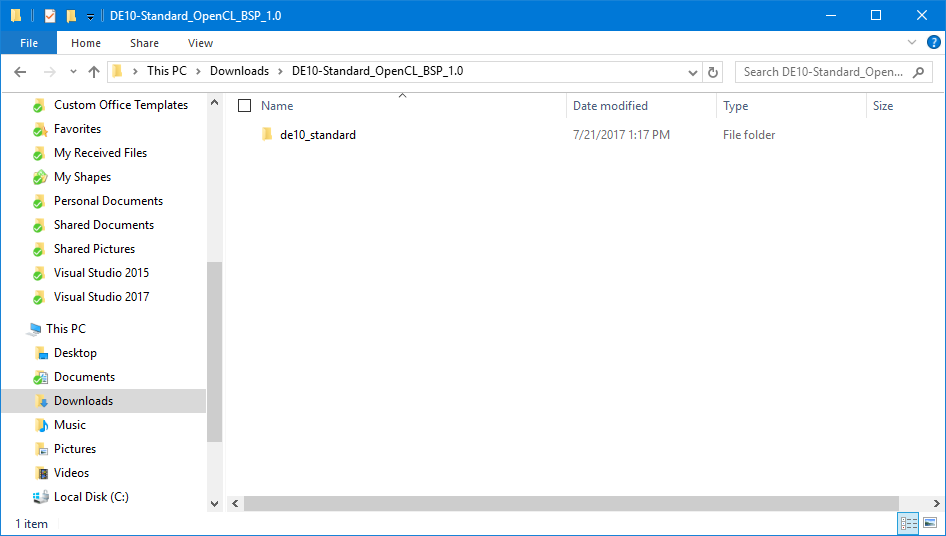
\includegraphics[scale = 0.7]{figures/fig_bsp_download_subdir.png}
%	\end{center}
%	\caption{Board Support Package download subdirectory}
%	\label{fig:bsp_download_subdir}
%	\end{figure}
	
	\begin{figure} [H]
	\begin{center}
	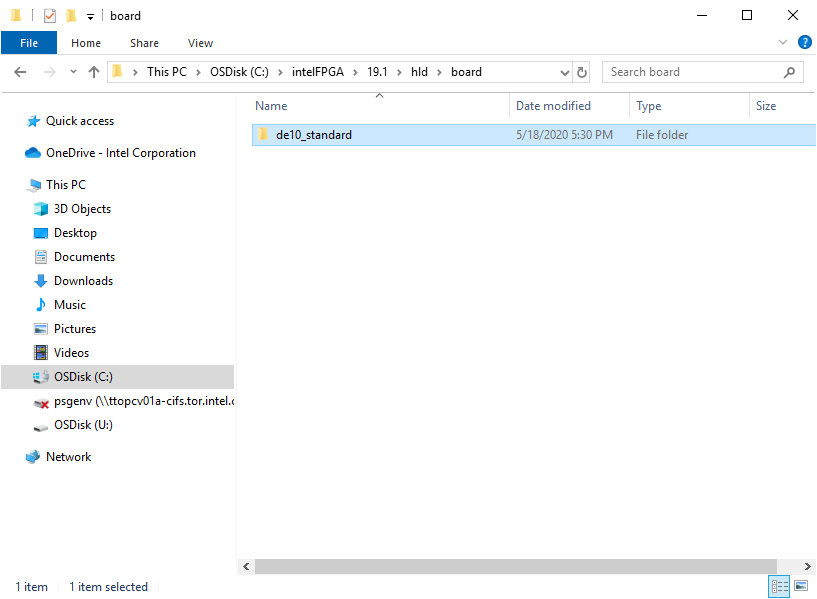
\includegraphics[scale = 0.6]{figures/fig_moving_bsp.png}
	\end{center}
	\caption{Extracting the Board Support Package to the \textit{<quartusroot>/hld/board/} Directory}
	\label{fig:move_bsp_download}
	\end{figure}
\item Create a new environment variable called \texttt{AOCL\_BOARD\_PACKAGE\_ROOT} and set its value to \\ \textit{<quartusroot>/hld/board/<extracted-bsp-directory>} (eg. \textit{C:/intelFPGA/\versnum/hld/board/de10\_standard}). In Linux you can set an environment variable by using the command \texttt{export <environment variable name>=<environment variable value>} in a terminal. In Windows you can set an environment variable by following the instructions in Section~\ref{sec:appendix_a}.
\item Ensure that the \texttt{AOCL\_BOARD\_PACKAGE\_ROOT}  points to a directory that contains a file named \textit{board\_env.xml}, as shown in Figure~\ref{fig:downloaded_bsp_directory}.
	\begin{figure} [H]
	\begin{center}
	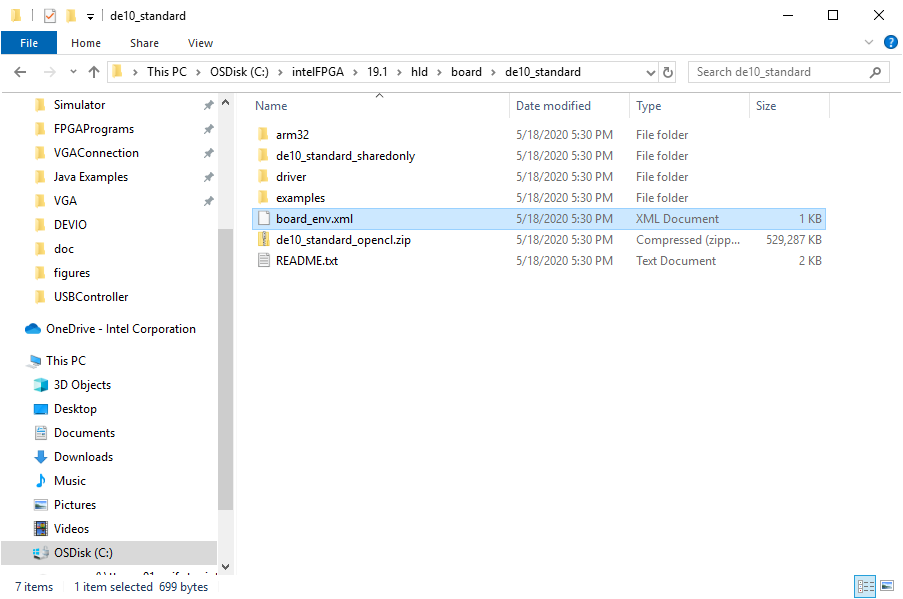
\includegraphics[scale = 0.6]{figures/fig_show_board_env.png}
	\end{center}
	\caption{Downloaded Board Support Package directory}
	\label{fig:downloaded_bsp_directory}
	\end{figure}
\item To test the board support package installation run the command \texttt{aoc -list-boards} in a Windows CMD prompt or a Linux terminal. 
The output should list the BSP that you just added, as shown in Figure~\ref{fig:verify_bsp_install} for the DE10-Standard.
	\begin{figure} [H]
	\begin{center}
	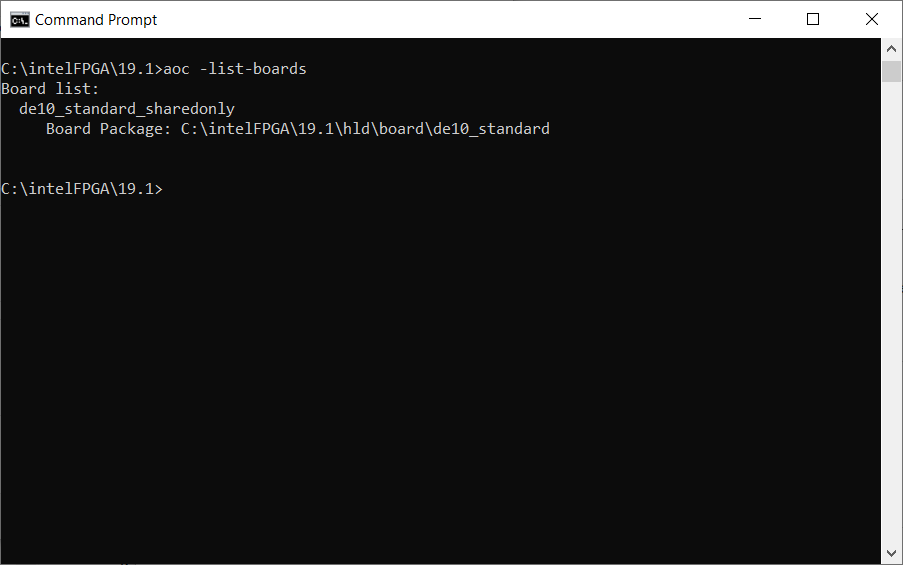
\includegraphics[scale = 0.5]{figures/fig_aoc_list_boards.png}
	\end{center}
	\caption{Verifying Board Support Package install}
	\label{fig:verify_bsp_install}
	\end{figure}
\end{enumerate}

For more instructions on installing board support, please refer to the \textit{Installing an FPGA Board} section of the document \href{https://www.altera.com/documentation/mwh1391807309901.html}{Intel SDK for OpenCL Getting Started Guide}.

\subsection{Setting up the Quartus and OpenCL SDK License File}

NOTE: As of version 17.1, you no longer require a license to use the Intel FPGA SDK for OpenCL. For prior versions, please refer to the instructions below.
The \texttt{INTELFPGAOCLSDKROOT} variable in the instructions below refers to the \textit{<quartusroot>/hld/} directory.

\label{sec:licensing}
If you have a \textbf{fixed} license follow these steps:
\begin{enumerate}
\item If you have a fixed license, copy the license (.dat) file to your local disk. A suggested location would be \textit{INTELFPGAOCLSDKROOT/licenses/} where you may have to create the \textit{licenses} directory in the \textit{INTELFPGAOCLSDKROOT/} directory.

\item Add or append to the \texttt{LM\_LICENSE\_FILE} environment variable, the path to your license file:\\
\textit{<path\_to\_license\_file>/<license\_filename>} (eg. \textit{INTELFPGAOCLSDKROOT/licenses/license.dat}).
\end{enumerate}

If you have a \textbf{floating} license follow these steps:
\begin{enumerate}
\item Obtain the the port number and host name from the network or system admin. Alternatively, the information is in the license file line \textsf{SERVER <hostname> <8 to 12 character host or NIC ID> <port>}.\\
The license for the user is \textsf{<port>@<hostname>}. If the port is not listed in the license file, specify \textsf{@<hostname>}.

\item Modify the license file to update the port number and host name.

\item Add or append to the \textit{LM\_LICENSE\_FILE} environment variable, the path to your license file: \path{<path_to_license_file>\<license_filename>} (eg. \path{INTELFPGAOCLSDKROOT\licenses\license.dat}).
\end{enumerate}

For more instructions on licensing the software, please refer to the \textit{Licensing the Software} section of the document \href{https://www.altera.com/documentation/mwh1391807309901.html}{Intel FPGA SDK for OpenCL Getting Started Guide}.

\section{Compiling an Example OpenCL\textsuperscript{\texttrademark} Application (Vector Addition)}
\label{sec:compiling}

\begin{figure} [H]
\begin{center}
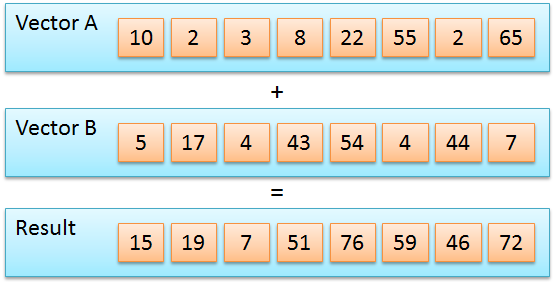
\includegraphics[scale = 0.7]{figures/vectoradd.png}
\end{center}
\caption{The Vector Addition OpenCL Application}
\label{fig:vector_add}
\end{figure}

In this section, we will compile the \textit{OpenCL Vector Addition Design Example} application for a DE-series SoC board. The source code for this design example can be downloaded at \href{https://www.altera.com/support/support-resources/design-examples/design-software/opencl/vector-addition.html}{https://www.altera.com/support/support-resources/design-examples/design-software/opencl/vector-addition.html}. This application performs vector addition of two vectors as shown in Figure~\ref{fig:vector_add}. More precisely, the application does the following:
\begin{enumerate}
\item The host program populates two arrays of equal length with randomized numbers. 
\item The host program computes the sums in software, using the CPU.
\item The kernel is used to compute the same additions again, using the FPGA.
\item The host program compares the results from the kernel to those that resulted from using the CPU. If the results are identical, the host program outputs the text "Verification: PASS" to indicate success. 
\end{enumerate}

\subsection{Compiling the Kernel}

We will first compile the kernel whose source code is located at \textit{/vector\_add/device/vector\_add.cl}. Compiling the kernel requires that the Intel FPGA SDK for OpenCL has been properly installed and configured, following the instructions in Sections \ref{sec:install_sdk} and \ref{sec:install_bsp}. You can compile the kernel by following the steps below:

\begin{enumerate}
%\item Extract the contents of the .tgz file to a directory of your choice.
\item Extract the contents of the \textit{exm\_opencl\_vector\_add\_arm32\_<version>.tgz} file to a directory of your choice.
\item In the commandline, navigate to the \textit{/vector\_add/} directory.
\item Compile the kernel by running the command (this can take some time):
\textbf{aoc device/vector\_add.cl -o bin/vector\_add.aocx -board=<target\_board>}
Where \textit{target\_board} is the board you installed in Section~\ref{sec:install_bsp}. The available boards can be list by running the following command:
	\textbf{aoc -list-boards}
\item The resulting Intel OpenCL Executable file \textit{vector\_add.aocx} is placed in the \textit{/vector\_add/bin/} directory.
\end{enumerate}

\subsection{Compiling the Host Program}

We will now compile the host program. Since the program will run on the ARM processor of the DE-series board, we must compile the host program code into an ARM binary. To do this, we will use the GNU toolchain included in the Linux distribution released for the DE-series board. This compilation process is referred to \textit{native compilation} since we are compiling the code on the same system that will run the binary. This is in contrast to \textit{cross-compiliation} which would be the process of compiling the binary on a non-ARM system (such as your x86 desktop or laptop) and then transferring the binary to the board to run it. To natively compile the host program, follow the instructions below:

\begin{enumerate}
\item Boot Linux on your board following the instructions in the tutorial \textit{Using Linux on the DE-Series Boards}.
\item Establish a commandline interface to the board either through USB-UART or SSH.
\item In the commandline, run the command \texttt{source /home/root/OpenCL/init\_opencl.sh} to configure the necessary environment variables.
\item Transfer the contents of the \textit{exm\_opencl\_vector\_add\_arm32\_<version>.tgz} file to a location of your choice on the board. For instructions on transferring files to the board's Linux file system, refer to Section \textit{Transferring Files to/from the Host Computer} in the tutorial \textit{Using Linux on the DE-Series Boards}.
\item In the commandline, navigate to the \textit{/vector\_add/} directory.
\item Compile the host program by running \textbf{make}. 
\item The resulting host program binary \textit{vector\_add} is placed in the \textit{/vector\_add/bin/} directory.
\end{enumerate}

%\subsection{Compiling the Host Program}

%We will now compile the host program. Since we want the host program to run on the ARM processor of the DE-series SoC board, we must cross-compile the program for the ARM architecture. To do this, we will use the \textbf{arm-linux-gnueabihf-} compiler toolchain. This toolchain is bundled with the Intel SoC EDS software suite, and can also be downloaded separately online (find it using your favorite search engine). Ensure that the \textit{bin} directory of the toolchain is added to your PATH environment variable (see \nameref{sec:appendix_a} for instructions on editing this variable), so that the toolchain is accessible from the command line. In addition, you will require the \textbf{gmake} utility, which can be downloaded online (again, make sure it is on your PATH). Once you have installed these tools, you can compile the host program using the steps below:

%\begin{enumerate}
%\item Extract the contents of the \textit{exm\_opencl\_vector\_add\_arm32\_<version>.tgz} file to a directory of your choice. The host program source code is located at \textit{/vector\_add/host/src/main.cpp}.
%\item In the commandline, navigate to the \textit{/vector\_add/} directory.
%\item Compile the host program by running \textbf{make}. 
%\item The resulting host program binary \textit{vector\_add} is placed in the \textit{/vector\_add/bin/} directory.
%\end{enumerate}

\section{Running OpenCL\textsuperscript{\texttrademark} Applications on DE-Series boards}
\label{sec:run_app}

OpenCL applications targeting DE-series SoC boards must run on top of the Linux operating system as they rely on Linux drivers that facilitate communication between the host program and the OpenCL kernel(s) inside the FPGA. This means that before you can run an OpenCL application, you must boot Linux on the board. The tutorial \textit{Using Linux on the DE-Series Boards} describes the process of booting Linux on DE-Series boards. Note that you must use a Linux distribution that contains support for OpenCL, such as the one used in the tutorial. Once you have booted up Linux, you can proceed to the following section.

\subsection{Running the Vector Addition OpenCL\textsuperscript{\texttrademark} Application}
\label{sec:run_application}

This section describes the steps for executing the \textit{Vector Addition} sample OpenCL program included with the DE-series Linux distribution. The commands shown are to be run in a commandline interface to the board, through a USB-UART or SSH connection. For instructions on establishing a commandline interface to the board, refer to the tutorial \textit{Using Linux on the DE-Series Boards}. 

To execute an OpenCL application, we must first run a script to setup the environment and load necessary OpenCL drivers. To do this, you can use the following command:

\begin{itemize}
\item[] \texttt{source /home/root/OpenCL/init\_opencl.sh}
\end{itemize}

Once we have executed the script, we can run the vector addition OpenCL application. For your convenience, the application comes preloaded in the Linux image. You can find the files \textit{vector\_add} and \textit{vector\_add.aocx} in \textit{/home/root/OpenCL/OpenCL\_Examples/vector\_add/}. Alternatively, if you compiled your own host program binary and aocx in Section~\ref{sec:compiling}, you can use them instead. To run the application, follow the instructions below:

\begin{enumerate}
\item Navigate to the directory:
\begin{itemize}
\item[] \texttt{cd /home/root/OpenCL/OpenCL\_Examples/vector\_add}
\end{itemize}
\item Program the FPGA with the kernel:
\begin{itemize}
\item[] \texttt{aocl program /dev/acl0 vector\_add.aocx}
\end{itemize}
\item Execute the host program:
\begin{itemize}
\item[] \texttt{./vector\_add}
\end{itemize}
\end{enumerate}

After running the commands listed above, you should see output similar to what is shown in Figure~\ref{fig:vector_add_commandline}. As shown in the figure, the host program executes, launching the kernel in the process. The host program displays the time taken in total as well as how much of the time was taken by the kernel. Finally, the host program compares the sums computed by itself to the sums computed by the kernel in the FPGA. If the sums match, the program outputs "Verification: PASS".

\begin{figure}[H]
   \begin{center}
       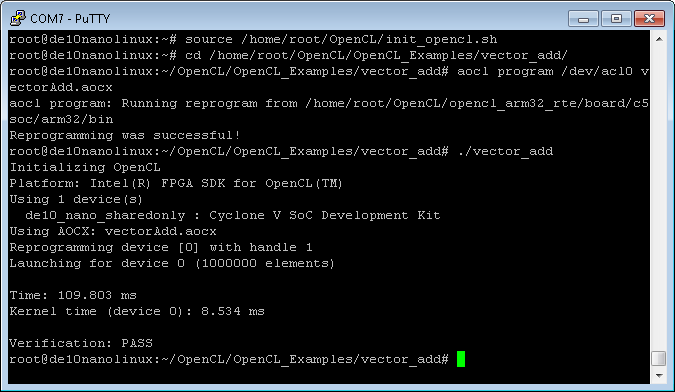
\includegraphics[scale=0.7]{figures/vectoraddcommandline}
   \end{center}
   \caption{Executing the vector addition application on the DE10-Nano board.}
	\label{fig:vector_add_commandline}
\end{figure}

\newpage
\section{Appendix A}
\label{sec:appendix_a}
\subsection{Adding and Editing Environment Variables in Windows*}
To add or edit environment variables first open the system control panel and navigate to \textsf{System > Advanced System Settings} to open the dialog window in Figure~\ref{fig:advanced_system_settings}.
	\begin{figure} [H]
	\begin{center}
	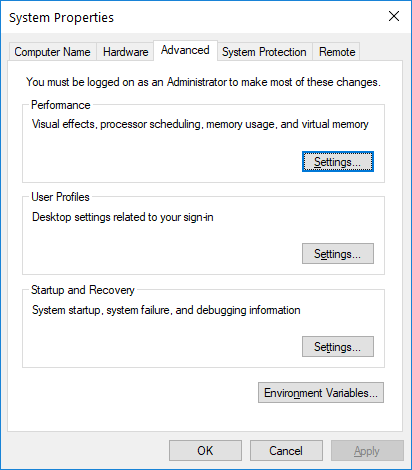
\includegraphics[scale = 0.7]{figures/fig_advanced_system_settings.PNG}
	\end{center}
	\caption{Advanced System Settings}
	\label{fig:advanced_system_settings}
	\end{figure}

From this dialog click \textit{Environment Variables...} to open the dialog in Figure~\ref{fig:env_vars}.
	\begin{figure} [H]
	\begin{center}
	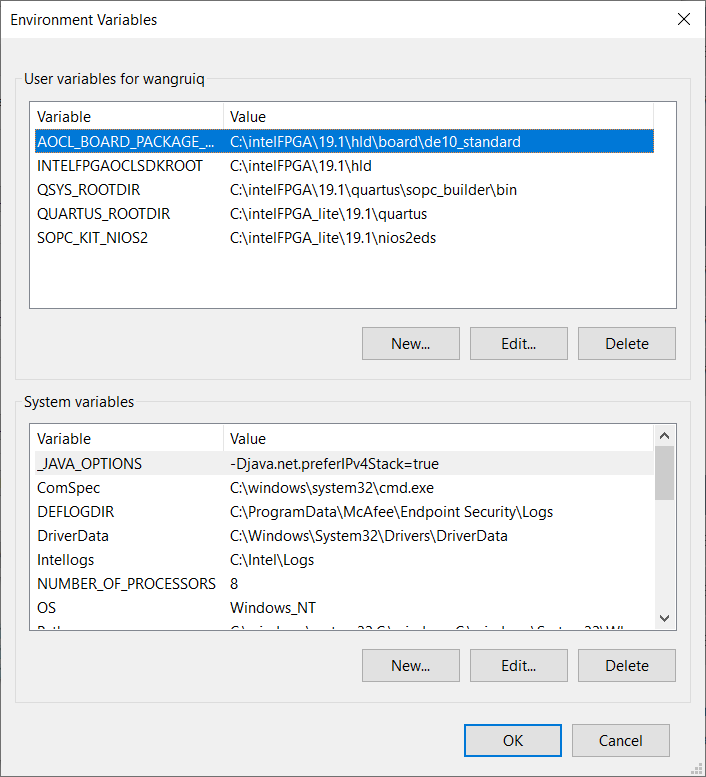
\includegraphics[scale = 0.7]{figures/fig_env_vars.PNG}
	\end{center}
	\caption{System Environment Variables}
	\label{fig:env_vars}
	\end{figure}
	
To edit the \textit{PATH} environment variable, select the \textit{Path} variable and click \textit{Edit} to open the dialog in Figure~\ref{fig:path_system_var}. From here you can add and remove paths.
	\begin{figure} [H]
	\begin{center}
	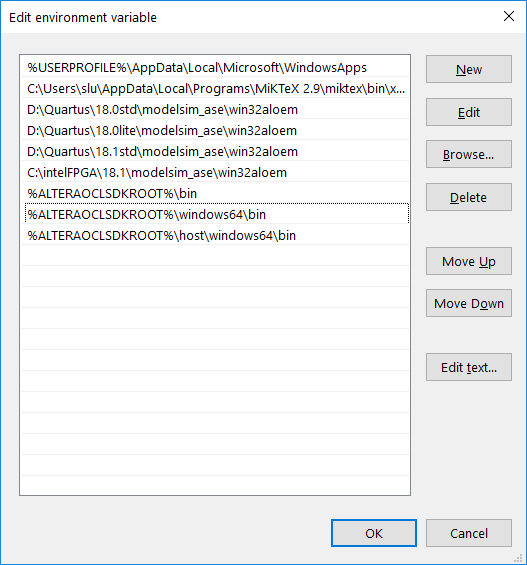
\includegraphics[scale = 0.5]{figures/fig_path_var.PNG}
	\end{center}
	\caption{'Path' System Environment Variable}
	\label{fig:path_system_var}
	\end{figure}

To add environment variables, click \textit{New...} in Figure~\ref{fig:env_vars} to open the dialog in Figure~\ref{fig:new_system_var}. From here you can define a new environment variable.
	\begin{figure} [H]
	\begin{center}
	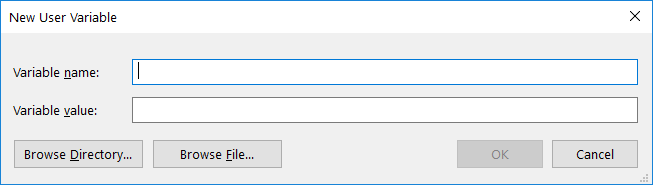
\includegraphics[scale = 0.7]{figures/fig_sys_settings_new_var.PNG}
	\end{center}
	\caption{New System Environment Variable}
	\label{fig:new_system_var}
	\end{figure}


% Copyright and Trademark


{\it OpenCL and the OpenCL logo are trademarks of Apple Inc. used by permission by Khronos.}
%\newcommand{\datePublished}{Mar 2022}

\newcommand{\versnum}{21.1} %version number quartus/AMP
\newcommand{\quartusname}{Quartus\textsuperscript{\textregistered} Prime}	
\newcommand{\textBar}{For \quartusname{} \versnum{}}
\newcommand{\thisyear}{2022 } %for copyright
\newcommand{\company}{FPGAcademy.org}
\newcommand{\longteamname}{FPGAcademy.org}
\newcommand{\teamname}{FPGAcademy}
\newcommand{\website}{FPGAcademy.org}

\newcommand{\productAcronym}{AMP}
\newcommand{\productNameShort}{Monitor Program}

\newcommand{\productNameMedTM}{Monitor Program}
\newcommand{\productNameMed}{Monitor Program}

%\newcommand{\headerLogoFilePath}[1]{#1/FPGAcademy.png}



%%%%%%%%%%%%%%%%%%%%%%%%%%%%%%%%%%%%%%%%
%%% FPGAcademy Copyright Information %%%
%%%%%%%%%%%%%%%%%%%%%%%%%%%%%%%%%%%%%%%%

%Always put the copyright on a new page (clear page), with some vertical space from top
\clearpage
\vspace{1in}

\noindent

Copyright {\copyright} FPGAcademy.org. All rights reserved. FPGAcademy and the FPGAcademy logo are trademarks of  FPGAcademy.org.  This document is being provided on an ``as-is'' basis and as an accommodation and therefore all warranties, representations or guarantees of any kind (whether express, implied or statutory) including, without limitation, warranties of merchantability, non-infringement, or fitness for a particular purpose, are specifically disclaimed.

%FPGAcademy assumes no responsibility or liability arising out of the application or use of any information,  product,  or  service  described  herein  except  as  expressly  agreed  to  in  writing  by  FPGAcademy.



**Other names and brands may be claimed as the property of others.




\end{document}

